% !TEX root = writing_version.tex

\label{chp:theory}

\section{Hard sphere system}
\label{sec:HS_system}
The hard sphere system is the simplest model of a fluid, going beyond the ideal gas only by including interactions between the particles in the form of an occupied volume. Its well known potential between particles i and j is given in \autoref{eqn:hs_potential}.
\begin{equation}
\label{eqn:hs_potential}
V(r_{ij})=%\infty \cdot \Theta(\sigma - r_{ij})
\begin{cases}
\infty \quad & r_{ij} \le \sigma \\
0 \quad & r_{ij} > \sigma
\end{cases}
\end{equation}
In this equation $r_{ij} = r_j - r_i$ denotes the distance between two particles and $\sigma$ is the diameter of a hard sphere.\\

While the ideal gas model without pair interactions already makes it possible to derive the famous equation of state $pV=NkT$, it does not include phase transitions yet. These can be observed when granting the particles space to occupy, in the simplest case by defining hard spheres of the kind in \autoref{eqn:hs_potential}. As it is the simplest model and it is efficiently accessible for computer simulations the hard sphere system is very well suited to study basic properties of first order phase transitions.\\ 

Compared to experiments where similar systems are realizable and extensively studied, general properties of the system at hand can be varied effortlessly and information about each single particle can be extracted easily as they are naturally required for the simulation.\\

On the downside computer simulations are much more constraint in their size, but with today's computational possibilities systems of the order of one million particles become tractable, and hence computer simulations are becoming an ever more powerful tool to study phase transitions of simple systems.\\

The first of such simulations date back to the beginning of electronic computer technology with first studies by Alder and Wainwright in 1959 \cite{Alders59}. Since then more algorithms to increase efficiency have been elaborated, and technology advanced to the point where virtual studies of large scale systems are possible.

\section{Memory effects and nucleation rates}
\label{sec:memory_approach}
Nucleation by itself can be characterized as a metastable state that, by crossing a first order phase transition, ends in a stable and qualitatively different state. Because nucleation processes are found in many circumstances, like atmosphere physics or metallurgy, people from various subjects have worked on understanding it.\\

Most descriptions are based on classical nucleation theory (CNT) which in a simple form is shown in \autoref{sec:CNT}. CNT is capable of qualitatively capturing the behaviour of nucleations, but often fails a quantitative comparison to experiments or numerical findings, sometimes by orders of magnitude. Models of this kind often include modifications to circumvent field specific problems but no broadly applicable framework has found a consensus to fully describe nucleations today\cite{MeyerThesis}.\\

\todo{include Markovian embedding?}\\

There are other theoretical works beyond the classical nucleation theory that not only tailor CNT to a specific problem but actually are based on more fundamental ideas. These take into account memory effects and non stationarity, where the latter is obviously important for phase transitions.\\

In the 1960's Mori and Zwanzig used their projection operator formalism to derive the Generalized Langevin equation while Grabert later also used a time dependent formalism introducing non stationarity. Based on these earlier works Meyer et al. derived the non stationary Generalized Langevin Equation (nsGLE)\cite{Meyer_nsGLE}. While the framework is too broad to cover at this point we may show the nsGLE in \autoref{eqn:EOM_A} to understand the memory kernel that is evaluated in \autoref{sec:memory_kernels}.
\begin{equation}
\label{eqn:EOM_A}
  \frac{d A_{t}}{dt} = \omega (t) A_{t} + \int_{0}^{t} K(\tau, t) A_{\tau} d\tau + \eta(0,t) \quad ,
\end{equation}
In the equation $A_{t}$ denotes an observable depending on time on a single trajectory, $\omega (t)$ is the time dependent friction coefficient, $\eta(0,t)$ is a time dependent noise term and $K(\tau, t)$ is the memory kernel depending on two times. As can be seen the memory kernel is integrated over, which means that it holds the information about how the history of the observable's trajectory influences its future. As the kernel depends on two times this impact is time dependent. Further we may note that Markovian processes exhibit a Dirac delta distribution, as they do not include memory, in which case \autoref{eqn:EOM_A} is reduced to the usual Langevin equation.\\

Quantifying the actual impact of memory effects in different systems is necessary for studying the use of the above mentioned ideas. For example Kuhnbold et al.\cite{Kuhnbold2019} have previously studied the nucleation process of a metastable Lennard-Jones fluid concluding that memory effects can not be neglected for an accurate description. One aim of this thesis therefore is to extend this picture by a study of memory effects in the nucleation of the metastable hard sphere fluid, done in \autoref{sec:memory_kernels}.\\

An other question concerning the hard sphere system is to measure nucleation rates which summarize by some definition how fast the phase transition occurs. 

An other major aim is to help understand the huge discrepancy between nucleation rates of the hard sphere system measured in experiments on the one hand and in computer simulations on the other hand. To explain the difference spanning order of magnitude, multiple attempt have been made but it could not be resolved until now. To this purpose a detailed analysis and characterization of the hard sphere nucleation process is done, leading to a speculation on the origin of the discrepancy.\\

\section{The phase diagram and the meta stable fluid}
\label{sec:HS_phase_diagram}
The equation of state for the monodisperse hard sphere system has various approximations \cite{Mulero2001}. The most common of these approximations due to its simplicity is the Carnahan-Starling approximation\cite{Carnahan1969}
\begin{equation}
\label{eqn:CS}
Z=\frac{1+\eta+\eta^2-\eta^3}{(1-\eta)^3} \; \text{.}
\end{equation}
It approximates the compressibility factor Z as a function of the packing fraction $\eta$ for the hard sphere fluid.\\

For the stable solid branch a common approximation is given by the Almarza equation of state\cite{Almarza2009}
\begin{equation}
\frac{p(v-v_0)}{k_B T} = 3 - 1.807846 y + 11.56350 y^2 + 141.6 y^3 - 2609.26 y^4 + 19328.09 y^5 \; \text{.}
\end{equation}
where p is the pressure, v is the volume per particle $v_0=\sigma^3/\sqrt{2}$ is the volume per particle at close packing, including the diameter of the spheres $\sigma$ and $y=p \sigma^3 / (k_B T)$, with $k_B$ being the Boltzmann constant and T the temperature of the crystal.\\
The inverse of the volume per particle corresponds to the number of particles per volume $ v^{-1} = \rho$. The relation to the corresponding packing fraction $\eta$ is given by $\rho = \frac{6}{ \pi} \eta$, which can be easily shown by extending $\rho = \frac{N}{V}$ by the single particle's volume $V_s = \frac{4}{3} \pi \left(\frac{\sigma}{2}\right)^3 = \frac{\pi}{6} \sigma^3$.\\
Within the thesis mostly but not only the volume fraction is used as it is the most common parameter for describing the system, but it can always be interchanged by the density.\\ 

A first order phase transition occurs when switching between the two stable branches of the system, described by the two equations of state, in between volume fractions of $\eta_{freeze} = 0.494$ and $\eta_{melt}=0.55$. They correspond to first solidifying clusters when approaching the transition from the liquid branch and melting of the crystalline phase when approaching the transition from the solid branch. Within this volume fraction interval the systems tends towards a coexistence state that in its equilibrium only varies the fraction of solid to liquid volume.\\
This can be understood in the following way: The liquid may follow its branch to pressures above the coexistence pressure. As it becomes unstable the particles may arrange into the crystalline phase as each single particle can access a larger free volume in the structured lattice than it would be possible in the unordered fluid.\\
By comparing the volume fractions of random close packing $\eta_{RCP}\approx 64\%$ with the one of a face centered cubic or hexagonal close packing fraction of $\eta_{HCP} \approx 74 \%$ this becomes evident. Within the crystalline phase each particle still has free volume accessible while the randomly packed particles are already confined at exactly one place.\\
This additional accessible volume translates into a larger number of possible states for the particle or in terms of thermodynamics a larger entropy, that acts as a driving force for the metastable fluid into the solid phase. As the particles in the crystal are packed more densely with a volume fraction of $\eta_{melt}=0.55$, the pressure is reduced and not all fluid transforms into the solid phase, but both phases may coexist.\\
The overall phase diagram is shown with the coexistence pressure in \autoref{fig:hs_phase_diagram}.\\

\begin{figure}[h]
\centering
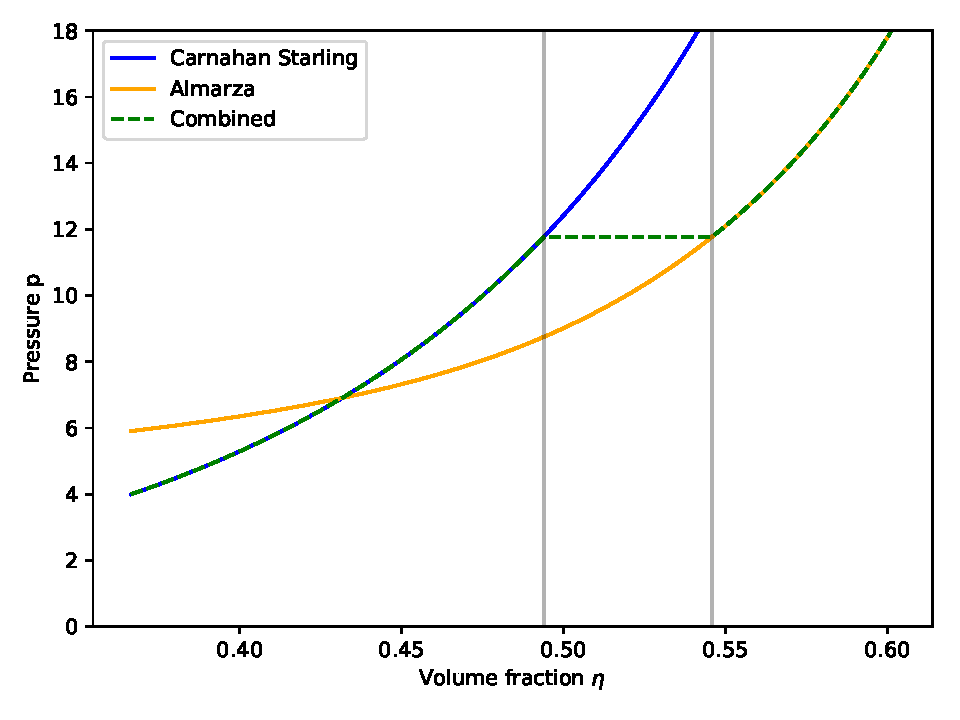
\includegraphics[width=0.6 \linewidth]{Hard_sphere_phase_diagram.pdf}
\caption[Hard sphere phase diagram]{Phase diagram of the hard sphere system with freezing and melting volume fraction shown as shaded lines and the green dashed line indicating the equilibrium stable branch. Where liquid and solid branch do not coincide with the stable branch these are unstable and tend towards the stable branch.}
\label{fig:hs_phase_diagram}
\end{figure}

The solid fraction in terms of volume for the system $x_s = \frac{V_s}{V}$ with $V_s$ the solid volume and $V$ the total volume can be described within the coexistence region in the equilibrium state by \autoref{eqn:solid_fraction}.\\ 
For the derivation it is necessary to use that in the stationary state the density of the solid phase is given by the melting density and that the liquid density is equal to the freezing density, i.e $\rho_s = \rho_{\text{melt}}$ and $\rho_l = \rho_{\text{freeze}}$ respectively.\\
When further using the trivial equations
\begin{align}
V &= V_s + V_l \; \text{,} \nonumber\\
N &= n_s + n_l \; \text{,} \nonumber\\
N_i &= \rho_i V_i \; \text{,} 
\end{align}

with $n_{s/l}$ the number of solid/liquid particles we may write

\begin{align}
\rho V &= \rho_s V_s + \rho_l V_l
\end{align}
leading under the assumption of equilibrium within a few lines of calculation to 
\begin{align}
\frac{V_s}{V} &= \frac{\rho - \rho_{\text{freeze}}}{\rho_{\text{melt}} - \rho_{\text{freeze}} } \; \text{.}
\end{align}
As the solid fraction below $\rho_{\text{freeze}} $ vanishes and above $\rho_{\text{melt}}$ is 1, we can conclude that the equilibrium solid fraction of the system is given by \autoref{eqn:solid_fraction_result}.
\begin{align}
\label{eqn:solid_fraction_result}
x_s(\rho) = 
\begin{cases}
0 & \rho <  \rho_{\text{freeze}}\\
\frac{\rho-\rho_{\text{freeze}}}{\rho_{\text{melt}}-\rho_{\text{freeze}}} &  \rho_{\text{freeze}} < \rho <  \rho_{\text{melt}}\\ 
1 &  \rho > \rho_{\text{melt}} \quad \quad \text{.}
\end{cases}
\end{align}

Evaluating the above result at feasible volume fractions for nucleation in between $\eta \in [0.53,0.55]$ leads to coexistence fractions of $x_s \in [0.7,1]$. This means that we are expecting nucleated systems to consist mostly of the solid phase after enough time for complete crystallization.\\

As pointed out earlier the phase transition takes place as it reduces the pressure in the liquid. This means that already during the growth of clusters the volume fraction of the metastable liquid is reduced, potentially altering its behaviour significantly. For closer inspection of this the particle density of the metastable liquid depending on the solid fraction $x_s$ is evaluated in \autoref{eqn:meta_stable_volume_fraction}. For this purpose first the liquid volume $V_l$ and the number of liquid particles $N_l$ are expressed in terms of the solid fraction $x_s$:
\begin{align}
\label{eqn:volume_relation}
V_l(x_s) & = V(1-x_s)\\
\label{eqn:number_relation}
N_l(x_s) & = N-n_s(x_s) = N - \rho_m V x_s = N(1-\frac{\rho_m}{\rho}x_s)
\end{align}
Combining \autoref{eqn:volume_relation} and \autoref{eqn:number_relation} to the expression for the particle density in the remaining liquid leads to
\begin{align}
\label{eqn:meta_stable_volume_fraction}
\rho_l(x_s) &= \frac{N_l (x_s) }{ V_l(x_s) } = \frac{N}{V} \frac{1-\frac{\rho_m}{\rho}x_s}{1-x_s} = \rho \frac{1-\frac{\rho_m}{\rho}x_s}{1-x_s}
\end{align}
Some examples of \autoref{eqn:meta_stable_volume_fraction} are depicted in \autoref{fig:remaining_density} for moderate solid fractions of the system at regular volume fractions used for nucleation.\\
\begin{figure}[h]
\centering
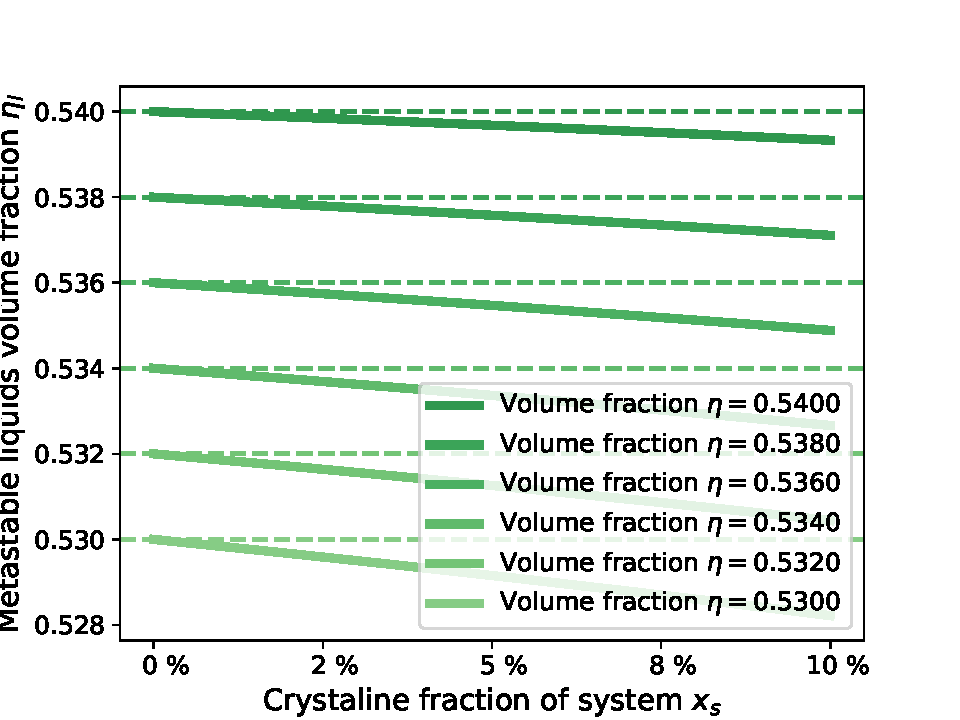
\includegraphics[width=0.5 \linewidth]{remaining_density.pdf}
\caption[Density decrease of the fluid during crystallization]{Visualization of \autoref{eqn:meta_stable_volume_fraction}. The volume fraction of the remaining liquid decreases for all shown initial volume fractions only little up to crystalline ratios of a few percent.}
\label{fig:remaining_density}
\end{figure}
What can be seen is that for crystalline fractions of a few percent the remaining liquid is not altered significantly. Especially for system sizes of about 1 million particles it already corresponds to cluster sizes of a few ten thousand particles, where stable growth of clusters takes place which is rather insensitive to changes of the volume fraction as shown in \autoref{sec:cluster_growth}. This means that during the highly sensitive cluster forming processes the volume fraction of the liquid can be assumed to be globally stable.\\ 

%Eventhough not further discussed in this thesis it might be said that for polydisperse radii the phase diagram becomes even richer as show for example in 
%\todo{https://journals.aps.org/prl/pdf/10.1103/PhysRevLett.91.068301}

\section{Classical nucleation theory }
\label{sec:CNT}
Classical nucleation theory (CNT) has been proposed by Becker and Döring in 1935\cite{Becker1935} and since then used and modified multiple times to suit various types of systems. Modifications of it are necessary to account for deviations off experimental results. Still it provides some reference or expectation to compare with the simulation data. Still its framework seems not to encompass the full process.\\

The simplest version of CNT assumes that a spherical crystallite may form in the liquid with properties of the bulk crystal while the fluid remains with the properties of the bulk liquid. The difference in the free energy landscape is given by a surface and a volume term. The first arises from the surface tension $\gamma$ between the fluid and the solid bulk phase. The latter is caused by the difference in chemical potential $\Delta \mu$. The whole expression for the free energy is given by
\begin{equation}
\label{eqn:free_energy}
\beta \Delta G(R) =4 \pi R \gamma -\frac{4}{3} \pi R^3 \rho \Delta \mu  \; \text{,}
\end{equation}
where $\rho$ is the particle density of the solid phase and further $R$ is the radius if the crystallite.\\

For the difference of the chemical potential $\Delta \mu $ we first derive the free energy difference between the metastable liquid branch and the stable coexistence branch. To calculate the free energy we employ its differential relation
\begin{align}
\label{eqn:differential_relation}
dF = -S  \, dT -P \, dV + \mu  \, dN
\end{align}
at a constant number of particles and constant temperature. By reformulating $dV$ using $ dN = dV  \, \rho + V  \, d\rho  $ and $dN = 0 $ we find  $ dV = -d\rho \frac{N}{\rho^2}$. Under this transformation \autoref{eqn:differential_relation} becomes
\begin{align}
\label{eqn:df_relation}
\frac{dF}{N} = \frac{P(\rho)}{\rho^2} d\rho \; \text{.}
\end{align}

The pressure $P(\rho)$ is given by the equation of state and approximated by the Carnahan-Starling approximation where $\eta = \frac{6 \rho }{\pi}$ and $Z=\frac{pV}{NkT} = \frac{p(\rho)}{\rho kT}$. Integrating \autoref{eqn:df_relation} between two densities $\rho_{1/2}$ leads to
\begin{equation}
\frac{\Delta F}{N} = \int_{\rho_1}^{\rho^2} \frac{kT}{\rho} \frac{1+\left( \frac{6 \rho}{\pi}\right) +\left( \frac{6 \rho}{\pi}\right)^2 - \left( \frac{6 \rho}{\pi}\right)^3}{\left( 1 - \frac{6 \rho}{\pi}\right)^3} d\rho \; \text{,}
\end{equation}
with the analytical solution
\begin{equation}
\int_{x_1}^{x_2} \frac{1+(ax) +(ax)^2 - (ax)^3 }{( 1 - ax )^3 \,  x} dx = \left. \frac{3-2ax}{(ax-1)^2} + \text{log}(x) \right|_{x=x_1}^{x_2} \; \text{.}
\end{equation}
Dropping the lengthy notation for $\eta = \left( \frac{6 \rho}{\pi}\right)$ we end up with
\begin{equation}
\frac{\Delta F}{N} = kT \left(  \frac{3-2 \eta_2}{(\eta_2 - 1)^2} - \frac{3-2 \eta_1}{(\eta_1 - 1)^2} + \text{log}\left( \frac{\eta_2}{\eta_1} \right) \right)
\end{equation}
The analytical solution is compared in \autoref{fig:free_energy_diff} with numerically found results which have been calculated before the analytical solution was found. The free energy difference is in the following identified with the difference in chemical potential $\Delta \mu$ as it is the driving force of the nucleation. \todo{is this justified like this?} \\

\begin{figure}[h]
\centering
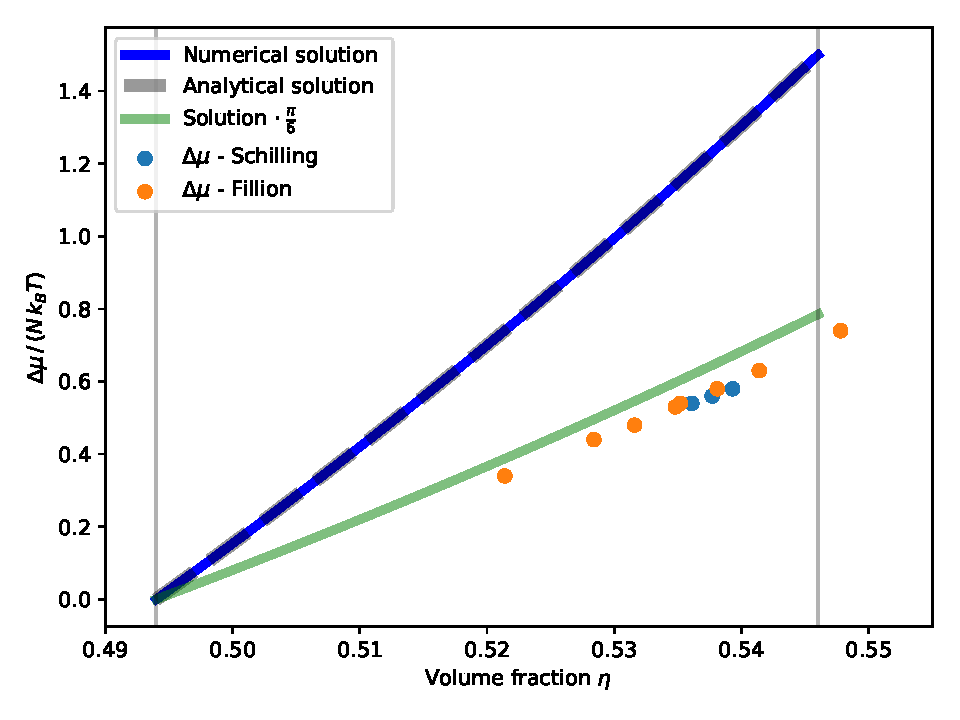
\includegraphics[width=0.7 \linewidth]{Free_energy_difference.pdf}
\caption[Free energy difference between fluid and solid phase]{Free energy difference per particle between the metastable liquid phase and the coexistence phase. Values found in the literature deviate from the shown result, but we assume that a factor of $\frac{\pi}{6}$ in the calculations is missing in either this or their calculation, as the modified green curve collapses rather accurately on the literature values when choosing $\eta_{freeze}=0.5$.}
\label{fig:free_energy_diff}
\end{figure}


Coming back to the free energy landscape of \autoref{eqn:free_energy} we see that it exhibits a maximum at a radius called $R_{crit}$. The interpretation of this radius is that if a cluster surpasses the critical radius it is likely to continue to grow until the system settles at the equilibrium solid fraction. Cluster in this sense is defined as a structure having a crystalline like ordering locally. The critical radius, simply calculated by setting the derivative of \autoref{eqn:free_energy} to zero, is given by \autoref{eqn:r_crit}.

\begin{equation}
\label{eqn:r_crit}
R_{crit} = \frac{2 \gamma}{\rho \Delta \mu }
\end{equation}

Furthermore the height of the barrier can be calculated to be 
\begin{equation}
\beta \Delta G (R_{crit}) = \frac{16 \pi \gamma^3}{3 \rho^2 (\Delta \mu )^2} \; \text{.}
\end{equation}

The classical critical radius depending on the volume fraction is depicted in \autoref{fig:r_crit} for a first impression of the cluster sizes that we are expecting for nucleation. The interfacial surface tension is often given by $\gamma \approx 0.6 k_B T \sigma^{-2}$ but it's precise value is under debate. Thus we may stick to one of the recently calculated values of $\gamma = 0.589 k_B T \sigma^{-2}$\cite{Bultmann2020}. 
\begin{figure}[h]
\centering
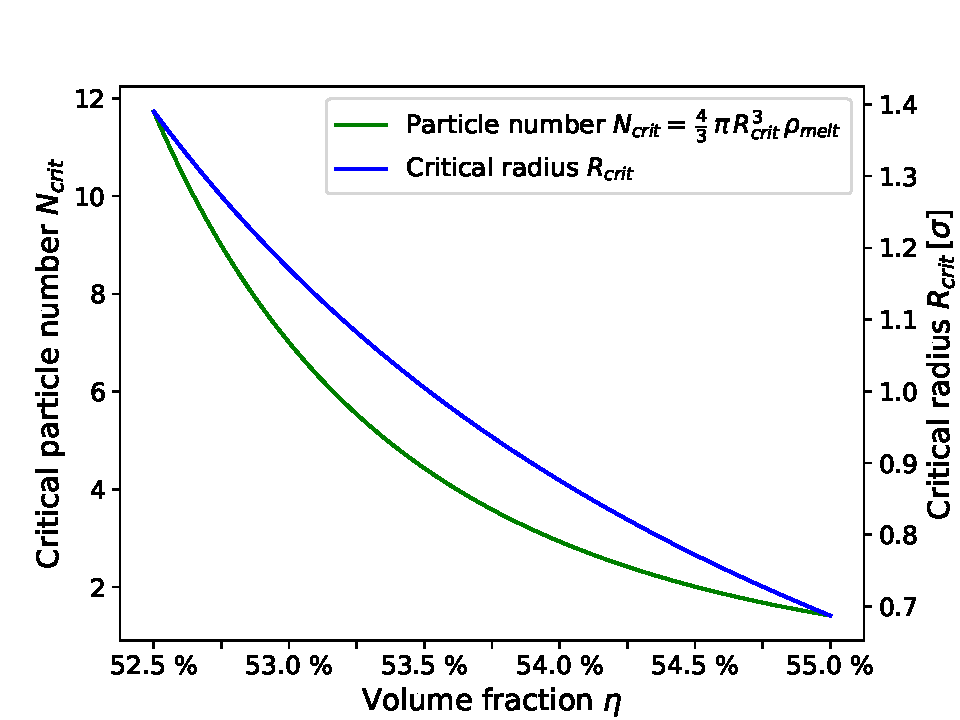
\includegraphics[width=0.7 \linewidth]{CNT_radius.pdf}
\caption[Critical radius in the metastable regime]{Critical radius $R_{crit}$ calculated from CNT depending on volume fraction $\eta$. As it can be seen the critical radii are rather small. When using the chemical potential calculated by Fillion and Schilling the critical clusters sizes become of the order $N \approx 50$ at intermediate metastable volume fractions, which is much more in agreement with typical largest cluster fluctuations found in simulations.}
\label{fig:r_crit}
\end{figure}

\section{Computer Precision}
\label{sec:precision}
The finite floating point precision of computers impacts the outcome of a single simulations as the simulation itself constitutes a many body problem with chaotic behaviour. In this section it is shown that even smallest variations of positions for example, lead to radical changes of the simulation after a certain number of steps. It is used to emphasize the importance to rigorously save the simulation state if it is supposed to be restarted from file, or with changing measurement intervals.\\

The exponential growth of induced variations in a chaotic system can be visualized by comparing a reference simulation with a pertubred one. In \autoref{fig:chaotic_behaviour} the mean of the squared displacements of all particles is observed between such a pair of simulations. The perturbation consists of a slight push of $10^{-10} \sigma$ to one particle's position, comparable with missing some floating point precision during saveing and loading.\\

\begin{figure}[h]
\centering
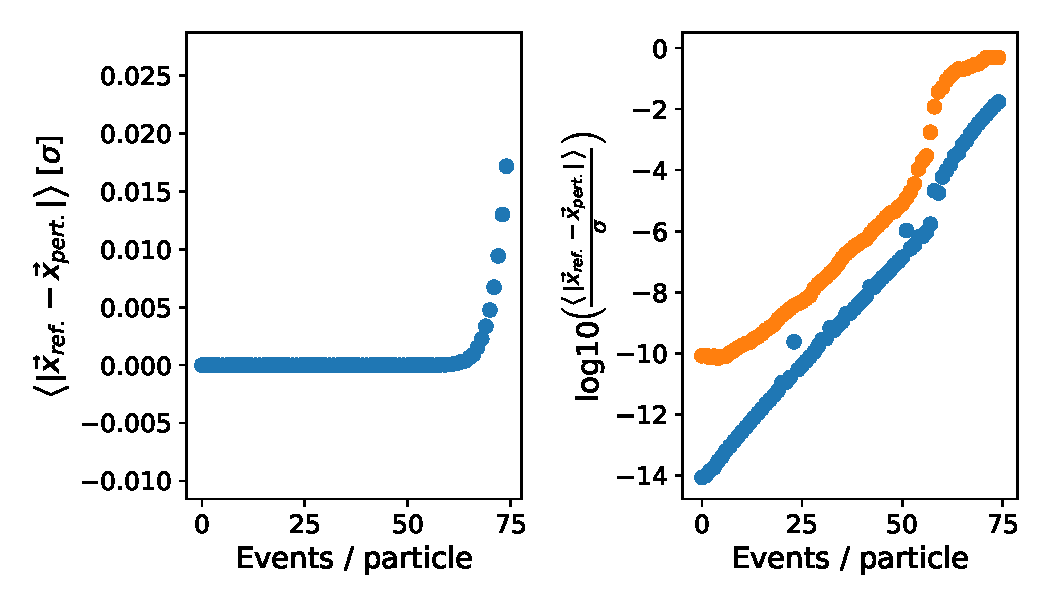
\includegraphics[width=0.6 \linewidth]{perturbation.pdf}
\caption[Exponential growth of perturbations in chaotic system]{Mean difference of particle positions in the reference and perturbed simulation. The blue lines show the same data while the orange curve shows the maximum deviation present at each step. For comparison with datasets using the system time $\delta t$ as units, a rough conversion is given by $T \approx \text{(\#steps)} \cdot \frac{1 \delta t}{60 \text{steps}}$ where a step is defined as one event per particle.\\ The maximum deviation first consists only of the initial perturbation but then increases similar like the mean deviation.}
\label{fig:chaotic_behaviour}
\end{figure}

Only observing the left side leads to the assumption that the simulations remain the same to a certain point and then suddenly diverge. But when looking at the logarithmic representation we see that actually the perturbation grows exponentially as long as it is small and deviates from this exponential growth at some point when reference and perturbed simulation become more or less independent of each other.\\
The small bumps at first sight seemed to be an artifact of the periodic boundary conditions but this seems not to be the case. What causes these deviations therefore remained hidden.\\

The challenge that this behaviour poses is that any perturbation leads to a completely different simulation. In the context of EDMD simulations we can for example look at the case when a measurement of some quantity is performed. For this purpose all particles have to be propagated to the global time. To not perturb the system with this extra calculations, an exact copy of the particle positions has to be saved prior to the propagation. After the measurement this copy is then used to restore the unperturbed system.\\ 
Similarly recalculating an event for the FEL at some point of time is not possible as the outcome will vary in the last floating point digits. For this reason it becomes necessary to save all precalculated events of the simulation to be able to restart it from a file.\\
Facing this challenge makes it possible to for example resimulate some interesting part of a trajectory from some saved checkpoint with a higher measurement frequency to resolve more details. 


\section{Comparison to real world experiments} 
\label{sec:comparison}

Starting in 1986 with the experiments by Pusey and Megen \cite{Pusey1986} hard spheres have been synthesized in the lab. Today a large variety of systems is known to show hard sphere like behaviour, but still further systems are developed to better controll stability, sphere size or also to reduce the possible impact of charges on top of the spheres as the Coulomb interaction alters the behaviour of the system strongly. All of these system have in common, that the hard spheres are in a bath of a fluid, which surrounds them. Even though nucleation experiments have been done without gravity in space\cite{Doherty1998} usually the fluid's mass density has to be matched to the mass density of the hard spheres to prevent sedimentation. Further it is necessary for optical measurements to match the refractive index of the fluid and the spheres as otherwise it becomes opaque .\\

The absence of the bath in simple hard sphere simulations constitutes a large difference to the hard sphere systems in the laboratory. On the one hand it has been argued that it only introduces a difference of the diffusion time scale and is regularly compensated by normalizing all times with a characteristic diffusion time. On the other hand a discussion on the possibility of hydrodynamic effects changing the behaviour of the laboratory system compared to simulations is ongoing at the moment,\todo{citation of the pro and contra hydrodynamics?} and also the mode spectrum of the suspending fluid within the cavities between the dispersed spheres might have a more important role 
than expected.\\ 
Even though it is desirable to include the suspending fluid into simulations, the proliferation of particles often is not feasible as calculation times increase by orders of magnitude.\\

A further difference is given by the spatial extent and geometry of the simulation. The geometry is often defined by periodic boundary conditions (PBC) in simulations to circumvent surface effects, but it is a rather unphysical setup.\\ 
Concerning the spatial extent, simulations are mostly confined to very small systems in comparison to experimental setups leading to a further difference between the measurement geometries. While the experimentalists usually probe a continuous volume of hard spheres in a suspending fluid, in simulations many disjunct volumes are used as each subvolume can be processed by one CPU. The expected behaviour of the disjunct volumes under the assumption of a constant nucleation rate is discussed in \autoref{sec:induction_time_expectation}. On the other side when not looking at ratios of nucleated and not nucleated boxes, but rather a quantity describing the overall solid fraction of a volume in the thermodynamic limit we may expect a different behaviour that is inspected in the following.\\

As is shown in \autoref{sec:cluster_growth} the cluster growth rate in simulations is more or less independent of the volume fraction. When making the assumption that this is the case not only in the small region in which it was tested, we may approximate the number of particles in a cluster $N$ at time $t$ as 
\begin{align}
N(t) = c^3 (t-t_0)^3 
\end{align} 
with $t_0$ the time where the cluster emerged from the fluid. Furthermore approximating the stochastic nucleation events by a constant rate at which new clusters are added to the system $\Delta t = (\kappa V)^{-1}$, we can write the total number of solidified particles $N$ in a Volume $V$ at time step $m$ with the corresponding time $t_m = m \Delta t$ as the sum of all previously nucleated cluster sizes $N_i$. Reformulating this leads to
\begin{align}
\begin{split}
N(t_m)&=\sum_{i=1}^m N_i\\
\Leftrightarrow N(t_m)&=\sum_{i=1}^m N_i \frac{\Delta t}{\Delta t}\\
\Leftrightarrow N(t_m)&=\kappa V \sum_{i=1}^m N_i \Delta t\\
\Leftrightarrow N(t_m)&=\kappa V \sum_{i=1}^m c^3 (t_m-t_i)^3 \Delta t
\end{split}
\begin{split}
\label{eqn:x_s_t_lim}
\stackrel{V \rightarrow \infty } {\Leftrightarrow} \quad N(t)&=\kappa V \int_0^{t} c^3 (t - t')^3 d t'\\
\Leftrightarrow \; \, \frac{N(t)}{V \rho_{\text{melt}}}&=\frac{\kappa c^3}{\rho_{\text{melt}}} \left. \frac{1}{4}t''^4 \right|_{t''=0}^t\\
\Leftrightarrow \; \; \; \; \frac{V_{solid}}{V} &= t^4 \frac{\kappa c^3}{4 \rho_{\text{melt}}}\\
\Leftrightarrow \quad \; \: x_s(t)&= t^4 \frac{\kappa c^3}{4 \rho_{\text{melt}}}
\end{split}
\end{align}
The solid fraction is not the equilibrium solid fraction, but rather the expected solid fraction of an infinitely large system at a time $t$ after some quench that suddenly takes the system into the metastable regime.\\ 
For the derivation of \autoref{eqn:x_s_t_lim} the thermodynamic limit $V\rightarrow \infty$ is used to obtain the definition of an integral. Further it neglects any interference between different clusters. This assumption is justified for $x_s \ll 1$ if no long range interference are present and heterogeneous nucleation is assumed to be part of the cluster growth process.\\

If the aforementioned assumptions also hold we can calculate a characteristic nucleation time $t^*$ at which $x_s$ is not negligible anymore. As in simulations with periodic boundary conditions clusters begin to interfere with each other at a filling fraction of about $x_s=\frac{1}{8}$ this is also chosen as a threshold where interferences can not be neglect any longer in the macroscopic system. Under this definition $t^*$ becomes
\begin{align}
\label{eqn:nucleation_time_modified}
t^* = \sqrt[4]{\frac{\rho_{\text{melt}}}{2 \kappa c^3 }} 
\end{align}
As we see the time $t^*$ actually depends only on the fourth root of the induction time $\tau_{nucleation} = \kappa^{-1}$. This might be an explanation for the huge discrepancy between experiment and simulation studies.\\

A first try is taken in \autoref{fig:nucleation_rate_comparison_modified}, where a nucleation time of the type defined in \autoref{eqn:nucleation_time_modified} is calculated and plotted together with other nucleation rates.
\begin{figure}[h]
\centering
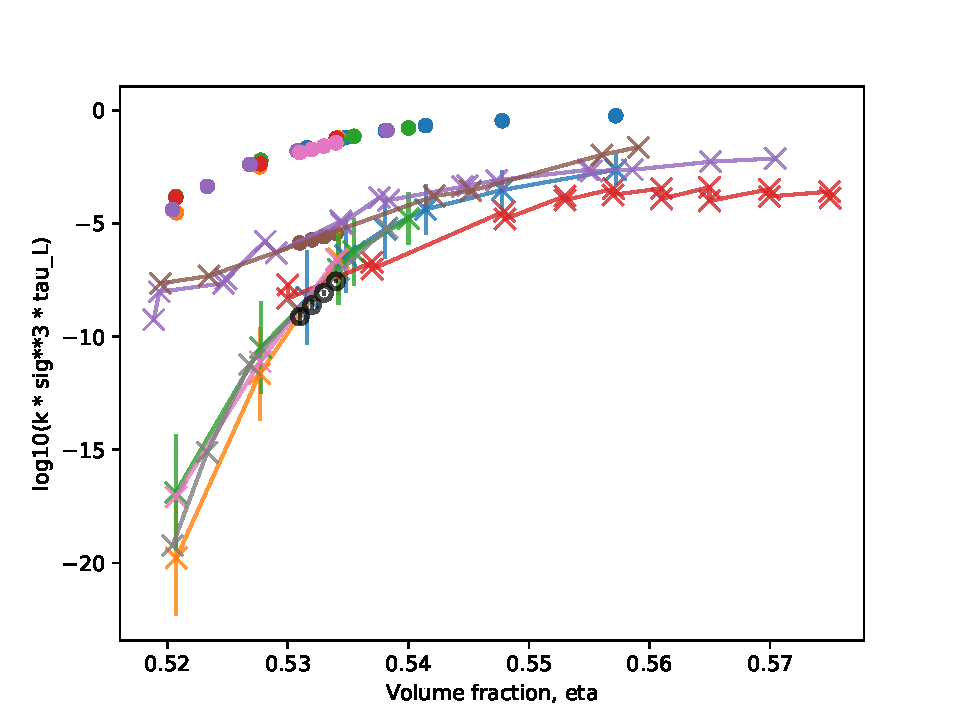
\includegraphics[width=0.6 \linewidth]{t_fill_rate_comparison.pdf}
\caption[Nucleation rate comparison under assumption of early filled boxes]{Diagram with modified nucleation rates calculated by \autoref{eqn:nucleation_time_modified}. The growth rate is set by the measurement shown in \autoref{sec:cluster_growth}. Furthermore a modified version with a factor 10000 is plotted to visualize the matching of the slopes. t\_fill denotes $t^*$ as it is the time until a significant fraction of volume is filled by clusters.}
\label{fig:nucleation_rate_comparison_modified}
\end{figure}
This can not be taken as a proof but as a hint that experimentalists might be measuring more cluster growth than nucleations. It has to be discussed with experimentalists if the assumptions leading to this result hold under close inspection or if measures against this behaviour have been taken like using many disjunct cavities.



